% ---------------------------------------------------------------------------
% Incremental, Multi-GPU CORE-SG -- IEEE Access format.
%
% Requires ieeeaccess.cls, which ships in the IEEE Access template package and
% is NOT part of TeX Live. Overleaf provides it. Place it beside this file for
% a local build.
%
% All figures are pgfplots/TikZ, so there are no external image dependencies
% and every plot is editable in place. Numbers come from results.csv (18,485
% measurements, 4x RTX 2080 SUPER) and results_local.csv (8,434, 1x RTX 4070 Ti
% SUPER); provenance is stated in Section V-A.
%
% TODO before submission: search for "TODO".
% ---------------------------------------------------------------------------
\documentclass{ieeeaccess}

% ---------------------------------------------------------------------------
% ieeeaccess.cls redefines the TeX primitive \year as a one-argument setter
% (\def\year#1{\gdef\theyear{#1}}, cls line 359), so \number\year no longer
% expands to a number. pgfmath initialises its random seed from it and fails
% with "Missing number, treated as zero" the moment pgfplots is loaded. Restore
% a numeric \year here; set the publication year through \theyear instead of
% \year{...}. Remove this block only if the figures stop using pgfplots.
% ---------------------------------------------------------------------------
\makeatletter
\let\accessyearsetter\year
\def\year{2026}          % TODO: publication year, also used by the page footer
\makeatother

% ---------------------------------------------------------------------------
% ieeeaccess.cls sets \xfigwd only inside its own \Figure macro (cls line 277),
% which wraps \includegraphics. Its \@makecaption then tests \ifdim\xfigwd
% (cls line 227), so ANY figure environment that is not an included image file,
% such as every TikZ or pgfplots figure here, fails with an undefined control
% sequence at the caption. Providing a zero default selects the ordinary
% column-width caption branch, which is correct for single-column figures. The
% class overwrites this whenever \Figure is used, so image figures are
% unaffected. Revisit if a full-width figure* is ever added.
% ---------------------------------------------------------------------------
\providecommand{\xfigwd}{0pt}

\usepackage{cite}
\usepackage{amsmath,amssymb,amsfonts}
\usepackage{algorithmic}
\usepackage{graphicx}
\usepackage{textcomp}
\usepackage{booktabs}
\usepackage{tikz}
\usepackage{pgfplots}
\pgfplotsset{compat=1.18}
\usetikzlibrary{arrows.meta,positioning}

\def\BibTeX{{\rm B\kern-.05em{\sc i\kern-.025em b}\kern-.08em
    T\kern-.1667em\lower.7ex\hbox{E}\kern-.125emX}}

\newcommand{\kmax}{k_{\max}}
\newcommand{\mpts}{m_{\mathrm{pts}}}
\newcommand{\mrd}{d_{\mathrm{mreach}}}
\newcommand{\coredist}{d_{\mathrm{core}}}

\begin{document}
\history{Date of publication xxxx 00, 0000, date of current version xxxx 00, 0000.}
\doi{10.1109/ACCESS.2024.DOI}

\title{Incremental, Multi-GPU Construction of the CORE-SG for Density-Based
Clustering at Scale}

% ---------------------------------------------------------------------------
% TODO: four authors. Replace names, memberships, affiliations and e-mails.
% ---------------------------------------------------------------------------
\author{\uppercase{First A. Author}\authorrefmark{1},
\uppercase{Second B. Author}\authorrefmark{2},
\uppercase{Third C. Author}\authorrefmark{3},
\uppercase{and Fourth D. Author}\authorrefmark{4},
\IEEEmembership{Member, IEEE}}

\address[1]{TODO Department, TODO University, TODO City, TODO Country
(e-mail: todo1@example.org)}
\address[2]{TODO Department, TODO University, TODO City, TODO Country
(e-mail: todo2@example.org)}
\address[3]{TODO Department, TODO University, TODO City, TODO Country
(e-mail: todo3@example.org)}
\address[4]{TODO Department, TODO University, TODO City, TODO Country
(e-mail: todo4@example.org)}

\tfootnote{TODO: funding and support acknowledgment.}

\markboth
{Author \headeretal: Incremental, Multi-GPU Construction of the CORE-SG}
{Author \headeretal: Incremental, Multi-GPU Construction of the CORE-SG}

\corresp{Corresponding author: First A. Author (e-mail: todo1@example.org).}

\begin{abstract}
Density-based clustering methods such as HDBSCAN* depend on a smoothing
parameter whose correct value cannot be known in advance, so a sweep over
candidate values is usually done. The CORE-SG replacement graph, the union of a
$k$-nearest-neighbour graph and one minimum spanning tree, removes the multiple
quadratic costs of that sweep by serving every smoothing value in a range
bounded by $\kmax$ from a single graph. It is, however, static and
single-machine: new data forces a full rebuild, and it does not fit within one
accelerator at scale. We make the CORE-SG incremental and multi-GPU by treating
its two constituent graphs separately. The neighbourhood graph is maintained by
dynamic NN-Descent decomposed into sampled instances, self-contained subproblems
that bound per-device memory and can be queued onto any accelerator. The
spanning tree is replaced by an anti-hub bridge estimate:
the only edges the neighbourhoods cannot supply are those bridging separated
components, such bridges leave from component borders, and spanning only the
nodes of lowest locally-normalised reverse degree suffices. That set is sized
independently of the number of points, so no spanning tree requires repair when
data arrives. Across 14 data sets and 18{,}485 measurements the estimate
yields spanning trees at most 0.024\% heavier than exact while producing
identical flat clusterings, and costs 10.5 to 36 times less. Incremental
construction exceeds a compute-matched rebuild by up to 7.0 percentage points of
recall, and on four GPUs an update reaches 3.23 times the single-device
throughput with per-device memory exactly invariant.
\end{abstract}

\begin{keywords}
Density-based clustering, GPU computing, hubness, incremental algorithms,
minimum spanning tree, nearest neighbour graph
\end{keywords}

\titlepgskip=-15pt

\maketitle

% ===========================================================================
\section{Introduction}
\label{sec:intro}
% ===========================================================================
\IEEEPARstart{D}{ensity-based} clustering does not operate on raw distances. It
first reweights the space by a local density estimate, and that estimate is
governed by a smoothing parameter, $\mpts$, that no principled procedure selects
in advance. Because no single value is appropriate for data whose components
differ in density, which is the usual case, it is common to sweep $\mpts$ and
inspect the resulting hierarchies. The cost of that sweep is steep, as the
clustering for a given $\mpts$ is determined by a minimum spanning tree (MST) of
a complete graph, and recomputing one per parameter value costs $O(n^2 d)$ each
time.

The CORE-SG replacement graph \cite{coresg} removes that barrier. A single
graph, built once, provably contains an MST of the complete
mutual-reachability graph for every $\mpts \le \kmax$. Extracting a clustering
then means reweighting $O(n\kmax)$ edges and running an MST over them, rather
than constructing a quadratic graph from scratch. The reported speed-ups are
large and we reproduce them.

Two properties of the original construction limit its reach: it is static and
single-machine. New data forces a full rebuild of both constituent structures.
And the MST, taken over the complete mutual-reachability graph, is $O(n^2 d)$ in
time and does not fit within one accelerator's memory at scale. Data that
arrives over time, common in the applications density-based clustering serves,
is therefore not supported.

\subsection{Contributions}

We make the CORE-SG incremental and multi-GPU. The central design decision is to
treat its two constituent graphs as separate problems, because they fail for
different reasons and admit different remedies.

\begin{enumerate}
\item \textbf{An incremental $k$-NN graph built from sampled instances.} Dynamic
      NN-Descent \cite{dynamic_nndescent}, our chosen strategy, refines a graph
      in place and is not incremental. We decompose each update into
      self-contained subproblems, each a random sample of the existing points
      merged with the whole arriving batch. Each instance is warm-started, bounds
      device memory to the size of its own sample plus the batch, and can be
      queued onto any accelerator without cross-device communication
      (Section~\ref{sec:knn}).

\item \textbf{An anti-hub bridge estimate replacing the MST.} The edges the
      neighbourhoods cannot supply are precisely those bridging density-separated
      components, and such bridges leave from component borders. We estimate
      borders by \emph{local inverse hubness}, a reverse degree normalised by the
      reverse degrees of one's own neighbours, which makes the statistic
      invariant to absolute density. Only the lowest-scoring nodes are spanned,
      and their number is fixed by the dimensionality and the edge count rather
      than by the number of points, so no spanning tree ever requires repair when
      data arrives (Section~\ref{sec:bridges}).
\end{enumerate}

% ===========================================================================
\section{Background and Related Work}
% ===========================================================================

\subsection{Density-Based Clustering and the Smoothing Parameter}

Given a data set $X \subset \mathbb{R}^d$ of $n$ points and a smoothing
parameter $\mpts$, the \emph{core distance} of a point $x \in X$ is the distance
from $x$ to its $\mpts$-th nearest neighbour,
\begin{equation}
\coredist^{\mpts}(x) = d(x, \mathrm{NN}_{\mpts}(x)),
\end{equation}
which is small in dense components and large in sparse ones. The
\emph{mutual reachability distance} \cite{hdbscan} between $x, y \in X$ is
\begin{equation}
\label{eq:mrd}
\mrd^{\mpts}(x,y) = \max\!\left\{\coredist^{\mpts}(x),\;
\coredist^{\mpts}(y),\; d(x,y)\right\},
\end{equation}
which inflates distances in sparse components while leaving dense ones
untouched, and thereby prevents single-linkage clustering from chaining through
noise.

The clustering itself is a spanning tree. Building the complete graph weighted
by $\mrd^{\mpts}$ and taking its MST yields a tree whose sorted edge weights are
exactly the merge heights of the single-linkage dendrogram; the HDBSCAN*
hierarchy is that dendrogram, and cutting it at a threshold $\varepsilon$
recovers the DBSCAN* clustering at $\varepsilon$ \cite{hdbscan_tkdd}, the
noise-aware variant of \cite{dbscan}. Flat clusterings are then extracted from
the hierarchy by stability maximisation \cite{fosc}. Everything downstream is
thus determined by one object, $\mathrm{MST}_{\mpts}$, and by the parameter that
defines it.

\subsection{The CORE-SG}

Neto et al. \cite{coresg} observe that a single graph can serve every $\mpts$ at
once. Define
\begin{equation}
\label{eq:coresg}
\mathrm{CORE\text{-}SG}_{\kmax} = \kmax\text{-}\mathrm{NNG} \;\cup\;
\mathrm{MST}_{\kmax},
\end{equation}
where $\mathrm{MST}_{\kmax}$ is the MST of the complete mutual-reachability
graph at the largest $\mpts$ of interest. Their Theorem~1 establishes that for
every $\mpts \le \kmax$, some MST of the complete $\mrd^{\mpts}$ graph is
contained in \eqref{eq:coresg}. Extracting $\mathrm{MST}_{\mpts}$ therefore
requires only reweighting the $O(n\kmax)$ stored edges with $\mrd^{\mpts}$ and
running an MST over that list.

This motivates our replacement of the second constituent graph. By
\eqref{eq:mrd}, an edge's weight falls into two cases. When $d(x,y)$ for
$x, y \in X$ is small relative to the two core distances, the weight is
determined by the core distances alone, which are recoverable from the $k$-NN
graph. The edges carrying information not already present are those where the
inter-point distance dominates both core distances: long edges bridging
components the neighbourhoods cannot reach. $\mathrm{MST}_{\kmax}$ supplies
those.

\subsection{Approximate $k$-NN Graph Construction}

NN-Descent \cite{nndescent} builds an approximate $k$-NN graph from the
principle that a neighbour of a neighbour is a likely neighbour, converging in a
few rounds of local joins. Dynamic NN-Descent \cite{dynamic_nndescent} samples
directly on the live graph, bounds the reverse-neighbour cache, and removes the
synchronisation requirement inside a round, which makes it amenable to
lock-free parallel execution. Neither is incremental in the sense of this study.
Both refine a whole graph in place, so inserting a batch either leaves the new
points without the neighbourhood structure the descent needs, or costs $O(n)$
per batch.

\subsection{Incremental and Streaming Density-Based Clustering}

FISHDBC \cite{fishdbc} is the closest published work. While it maintains a
spanning tree, we avoid it, which makes the algorithm a coherent baseline. It
is fed by candidate edges from a hierarchical navigable small world index
\cite{hnsw}. It also approximates HDBSCAN* for a single $\mpts$ only, and thus,
the multiple-$\mpts$ capability of the CORE-SG has no equivalent there.
I-HASTREAM \cite{ihastream} maintains a hierarchy over micro-clusters, a
different granularity, as do summarisation approaches such as Data Bubbles
\cite{databubbles} and BIRCH-derived methods \cite{birch}. Zubaro\u{g}lu and
Atalay \cite{streamreview} survey the wider stream-clustering field.

Closest to our $k$-NN graph is the work of Zhao et al. \cite{knn_merge} on
merging $k$-NN graphs, which also supports expanding an existing graph with a
raw data set and therefore addresses incremental construction directly. Our
merge step relies on the same idempotence of top-$k$ insertion; the difference
is that we decompose an \emph{update} into independent instances in order to
bound per-device memory, rather than combining independently built graphs.

On scalability rather than incrementality, distributed batch constructions
\cite{mrhdbscan} parallelise HDBSCAN* over MapReduce, McInnes and Healy
\cite{acceleratedhdbscan} accelerate it via spatial indexing, and Gowanlock
\cite{bpshdbscan} reaches billion-point DBSCAN with a hybrid CPU/GPU scheme.
None of these maintains a structure under insertion, and none serves a range of
$\mpts$ from a single graph. General dynamic MST maintenance
\cite{mst_maintenance} is well studied; we discuss in
Section~\ref{sec:bridges} why we avoid it.

\subsection{Hubness}

The asymmetry of the $k$-NN relation in high dimensions, where some points
appear in many neighbour lists while others in few, is a well-documented
phenomenon \cite{hubs}, usually studied as a problem. The reverse quantity has
been used for influence analysis \cite{influencesets} and supported by dedicated
index structures \cite{rdnntree}. We use it constructively: the \emph{low} end
of the reverse-degree distribution, normalised locally, estimates component
borders, which is where the edges we need originate.

% ===========================================================================
\section{Method}
\label{sec:method}
% ===========================================================================

Fig.~\ref{fig:pipeline} shows the pipeline. A batch of arriving points passes
through three stages. First, the $k$-NN graph is updated by sampled-instance
descent: each instance pairs its own random sample of the existing points with
the whole batch, the instances are merged into the global neighbour lists, and a
final restricted descent runs over the new points together with their
neighbourhood \emph{rings}, that is, their neighbours (ring 1) and their
neighbours' neighbours (ring 2). Second, the hubness index is refreshed over the
affected region and re-selects the anti-hubs, whose number is
$\lceil d \ln |E| \rceil$ for ambient dimensionality $d$ and undirected edge
count $|E|$ of the current $k$-NN graph. Third, a spanning tree is computed over
those anti-hubs to give the bridge edges, followed by a \emph{repair} step that
spans any components the bridges left disconnected, so that the result is always
a spanning tree rather than a forest. A query for $\mathrm{MST}_{\mpts}$ then
reweights the union with $\mrd^{\mpts}$ and runs a spanning-tree algorithm over
$O(n\kmax)$ edges.

\begin{figure}[!t]
\centering
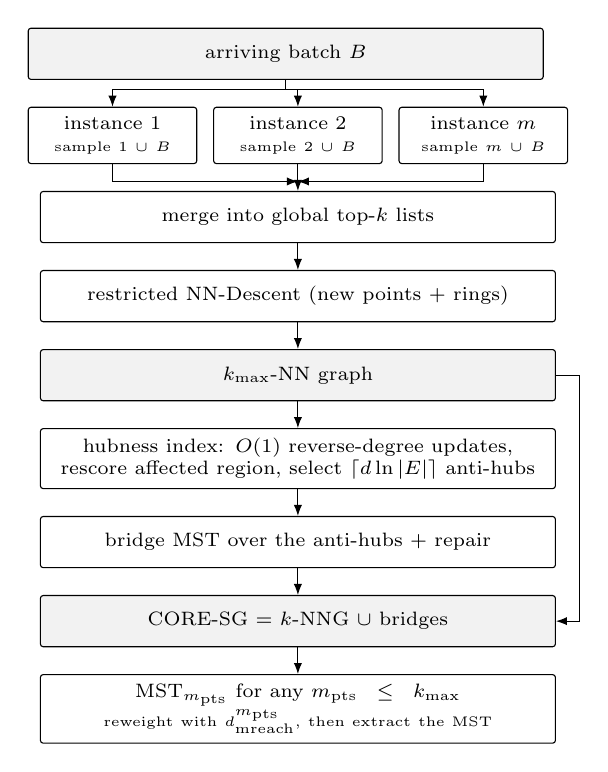
\begin{tikzpicture}[
  node distance=3.4mm,
  box/.style={draw, rounded corners=1pt, align=center, font=\scriptsize,
              minimum height=6.5mm, inner xsep=2pt, text width=20mm},
  wide/.style={box, text width=64mm},
  ar/.style={-{Latex[length=1.4mm]}, thin}
]
\node[wide, fill=black!5] (batch) {arriving batch $B$};
\node[box, below=of batch.south west, anchor=north west] (i1) {instance 1\\{\tiny sample 1 $\cup$ $B$}};
\node[box, right=2mm of i1] (i2) {instance 2\\{\tiny sample 2 $\cup$ $B$}};
\node[box, right=2mm of i2] (i3) {instance $m$\\{\tiny sample $m$ $\cup$ $B$}};
\node[wide, below=of i2] (merge) {merge into global top-$k$ lists};
\node[wide, below=of merge] (refine) {restricted NN-Descent (new points $+$ rings)};
\node[wide, below=of refine, fill=black!5] (knn) {$\kmax$-NN graph};
\node[wide, below=of knn] (hub) {hubness index: $O(1)$ reverse-degree updates,\\rescore affected region, select $\lceil d\ln|E|\rceil$ anti-hubs};
\node[wide, below=of hub] (br) {bridge MST over the anti-hubs $+$ repair};
\node[wide, below=of br, fill=black!5] (sg) {CORE-SG $=$ $k$-NNG $\cup$ bridges};
\node[wide, below=of sg] (out) {$\mathrm{MST}_{\mpts}$ for any $\mpts \le \kmax$\\{\tiny reweight with $\mrd^{\mpts}$, then extract the MST}};

\draw[ar] (batch.south) -- ++(0,-1.2mm) -| (i1.north);
\draw[ar] (batch.south) -- ++(0,-1.2mm) -| (i2.north);
\draw[ar] (batch.south) -- ++(0,-1.2mm) -| (i3.north);
\draw[ar] (i1.south) |- ([yshift=1.2mm]merge.north);
\draw[ar] (i2.south) -- (merge.north);
\draw[ar] (i3.south) |- ([yshift=1.2mm]merge.north);
\draw[ar] (merge) -- (refine);
\draw[ar] (refine) -- (knn);
\draw[ar] (knn) -- (hub);
\draw[ar] (hub) -- (br);
\draw[ar] (br) -- (sg);
\draw[ar] (knn.east) -- ++(3mm,0) |- (sg.east);
\draw[ar] (sg) -- (out);
\end{tikzpicture}
\caption{The update pipeline. Instances are independent subproblems and are the
unit of parallelism; only the merge and the bridge spanning tree are global, and
both operate on objects far smaller than the data set.}
\label{fig:pipeline}
\end{figure}

\subsection{The $k$-NN Graph: Sampled Instances}
\label{sec:knn}

An \emph{instance} is a random sample of the existing base points unioned with
the entire arriving batch, together with the edges those sampled points already
possess. Each instance is a self-contained NN-Descent problem with no reference
to global state, which yields three consequences.

Sampled base points arrive with real neighbourhoods, so an instance converges in
fewer rounds than a cold build. It bounds device memory to the size of its own
sample plus the batch rather than the whole data set, which admits data sets
larger than one accelerator. And instances never communicate, so they queue onto
whatever device is free; \emph{the instance count, not the device count, is the
unit of parallelism}, verified in Section~\ref{sec:scaling}.

After the instances complete, their neighbourhoods are merged into the global
graph by repeated insertion into sorted top-$k$ lists. This operation is
commutative and associative, meaning the merged result does not depend on the
order in which instances finish or on how their results are grouped, and
idempotent, meaning that merging the same neighbourhood twice changes nothing.
Instances may therefore complete in any order. A final NN-Descent restricted to
the new points and their neighbourhood rings repairs edges the sampling missed.

The refinement set is built as new points, then ring 1, then ring 2, and is
capped: unbounded it reaches $\Theta(k^2)$ nodes per new point. The cap
truncates the outermost ring first and never discards a new point. We
characterise its effect in Section~\ref{sec:sensitivity}.

\subsection{The MST: Anti-Hub Bridges}
\label{sec:bridges}

Maintaining an MST under insertion is possible \cite{mst_maintenance} but
costly, and the tree being maintained here is over a \emph{complete} graph whose
$O(n^2)$ edge weights all shift when $\mpts$ changes. We therefore estimate it.

Recall from \eqref{eq:mrd} that the MST need only supply edges bridging
density-separated components. Such a bridge leaves a component from its
\emph{border}, since an interior point always has a nearer neighbour in the
direction of travel. Estimating borders geometrically is awkward beyond low
dimensions; local inverse hubness estimates them directly. Define, for a node
$v$ of the $k$-NN graph with neighbour set $\mathrm{NN}(v)$,
\begin{equation}
\label{eq:rd}
\mathrm{rd}(v) = |\{ u : v \in \mathrm{NN}(u) \}|,
\end{equation}
the \emph{reverse degree}, that is, the number of nodes that list $v$ among
their own $k$ nearest neighbours, and
\begin{equation}
\label{eq:score}
\mathrm{score}(v) = \frac{\mathrm{rd}(v)}
     {\frac{1}{|\mathrm{NN}(v)|}\sum_{u \in \mathrm{NN}(v)} \mathrm{rd}(u)},
\end{equation}
the reverse degree of $v$ divided by the mean reverse degree over $v$'s own
neighbours. An interior point sits inside many of its neighbours'
neighbourhoods; a border point sits inside few, because its neighbours' lists
point back into the component. The denominator is what makes \eqref{eq:score}
usable: comparing $\mathrm{rd}(v)$ against the global population would merely
find sparse components, whereas comparing it against $v$'s own neighbourhood
makes the score invariant to local density. A border point of a dense component
scores like a border point of a sparse one, which is required when the data
mixes densities. Values below 1 indicate a local anti-hub.

The estimate is then: select the $\lceil d \ln |E| \rceil$ lowest scorers and
compute an exact MST over that set in mutual-reachability space. Its edges
become the bridges, stored with their base distance so that the reweighting for
a query $\mpts$ treats them identically to $k$-NN edges.

The size of the selected set depends on $d$ and $|E|$, \emph{not on $n$}. The
bridge computation is therefore $O(m^2 d)$ for $m$ selected anti-hubs with
$m \ll n$, and \textbf{no spanning tree requires repair when points arrive}.

Two properties of the implementation are worth stating. The hubness index
attaches to the $k$-NN graph as an observer, so every inserted or evicted
directed edge updates a reverse degree in $O(1)$ and marks the affected nodes; a
refresh rescores only the affected region rather than all $n$ nodes. And
although \eqref{eq:score} is defined over reverse neighbourhoods, the running
structure stores only a reverse \emph{degree} per node, an integer, never the
reverse-neighbour lists themselves.

\subsubsection{Component Coverage}

The anti-hub count $\lceil d \ln |E| \rceil$ is a function of dimensionality and
edge count only, and is therefore blind to how many density-separated components
exist. Once the number of components approaches that count, some components
receive no anti-hub at all and no bridge can leave them; we measured 120
components at $d=8$ fragmenting into 41 pieces. A \emph{per-component quota}
guarantees that every $k$-NN component contributes at least a fixed number of
its own lowest scorers, in addition to those selected globally. In a small
uniform detached component every node is exactly neutral under \eqref{eq:score},
so no score ranking reaches it however detached it is; bucketing by component
sidesteps the score entirely.

\subsubsection{Connectivity Repair}

An estimate can still leave the graph disconnected, which yields a forest rather
than a spanning tree. A repair step spans any remaining components using
anti-hubs drawn from each; contracting a connected spanning subgraph stays
connected, so retaining only the inter-component edges of the anti-hub MST
suffices.

Both mechanisms require knowing the components of the $k$-NN graph, which is
therefore on the critical path of every update. The labelling is obtained by a
lock-free union-find pass directly over the adjacency arrays, spread across a
thread pool, which costs 1 to 2\,ms at $n = 100{,}000$; folding the bridges into
the cached labels afterwards is $O(n + |\text{bridges}|)$. This is small against
the rest of an update, and Section~\ref{sec:connectivity} quantifies it against
the bridge computation it guards.

% ===========================================================================
\section{Experimental Setup}
\label{sec:setup}
% ===========================================================================

\subsection{Ground Truth: The Exact CORE-SG}

Every quality claim is measured against the \emph{exact} CORE-SG, an exact
$k$-NN graph by brute force plus an exact $\mathrm{MST}_{\kmax}$, and never
against human class labels. The claim under test is that an approximation
matches the object it approximates. Scoring against class labels would instead
measure whether HDBSCAN* suits a given data set, which is a problem out of this
work's scope.

\subsection{Metrics}

We report $k$-NN recall, the fraction of true $k$ nearest neighbours present in
the approximate graph; MST total weight ratio, approximate over exact; the
largest gap between the two sorted weight profiles, which measures dendrogram
similarity, since single-linkage merge heights \emph{are} the sorted MST
weights; and DBSCAN* ARI \cite{ari} between the flat clusterings cut from both
trees at a common threshold.

Two further quantities need definition. The \emph{component count of the $k$-NN
graph before repair} is the number of connected components the neighbourhood
graph falls into on its own, with no bridges added and no repair applied; it
states how much work the bridges have to do, and a value of 1 means they have
none. The \emph{phase-split wall clock} decomposes an update into the instance
descent, the merge, the restricted refinement, the hubness refresh, the bridge
MST and the connectivity pass, so that the parallel portion can be separated
from the sequential remainder.

We deliberately do \emph{not} report edge overlap between spanning trees. All
MSTs of a graph share a weight multiset, and for any threshold the components of
the sub-threshold edge set depend on the graph rather than on which MST was
extracted, so two different MSTs induce very similar single-linkage hierarchies.
Measured on our system, overlap collapses from 0.99 to 0.19 as $\mpts$ rises
from 1 to 32 while ARI remains exactly 1.0000, because raising $\mpts$ flattens
the mutual-reachability landscape into plateaus of tied weights and any
tie-break yields a different but equally optimal tree.

\subsection{Data Sets}

Table~\ref{tab:datasets} lists the three families. \textbf{Real-paper} sets
reproduce the recipes of \cite{coresg} for comparability, using FMA \cite{fma}
and 20 Newsgroups \cite{newsgroups}. \textbf{Real-scale} sets exercise scale,
high dimensionality and a non-Euclidean metric: SIFT1M and GIST1M
\cite{sift_gist}, and GloVe \cite{glove} under cosine distance.
\textbf{Manifold} sets are synthetic, generated in a low dimensionality and
rotated into a high one by a random orthonormal map, which preserves every
pairwise distance exactly, so component structure and separation are untouched
while ambient dimensionality rises and intrinsic dimensionality is known by
construction.

The manifold family exists because of a finding we report in
Section~\ref{sec:connectivity}: no real data set we examined produces a
fragmented $k$-NN graph, so none of them can exercise the bridges at all.

\begin{table}[!t]
\caption{Data sets. ``comp.'' is the number of components of the $k$-NN graph
alone at the operating $\kmax$ (Section~\ref{sec:connectivity}), measured with
an \emph{exact} $k$-NN graph for the $n = 4{,}000$ sets, where the exact
reference is affordable and Table~\ref{tab:bridges} is computed, and with the
\emph{approximate} graph at full $n$ for the rest.}
\label{tab:datasets}
\centering
\footnotesize
\begin{tabular}{@{}llrrrr@{}}
\toprule
family & set & $n$ & $d$ & $\kmax$ & comp. \\
\midrule
real-paper & \texttt{fma\_chroma}   & 106{,}574 & 84   & 32 & 1 \\
           & \texttt{fma\_mfcc}     & 106{,}574 & 140  & 32 & 1 \\
           & \texttt{20ng\_tfidf}   & 10{,}969  & 1000 & 24 & 1 \\
           & \texttt{20ng\_pca500}  & 10{,}969  & 500  & 24 & 1 \\
\midrule
real-scale & \texttt{sift1m}        & 200{,}000 & 128  & 32 & 1 \\
           & \texttt{gist1m}        & 100{,}000 & 960  & 32 & 1 \\
           & \texttt{glove100}      & 200{,}000 & 100  & 32 & 1 \\
\midrule
manifold   & \texttt{manifold\_exact} & 4{,}000   & 128 & 24 & 16 \\
           & \texttt{manifold\_c8}    & 4{,}000   & 128 & 24 & 8  \\
           & \texttt{manifold\_c24}   & 4{,}000   & 64  & 24 & 24 \\
           & \texttt{manifold\_c32}   & 4{,}000   & 128 & 16 & 32 \\
           & \texttt{manifold\_mid}   & 100{,}000 & 128 & 24 & 132 \\
           & \texttt{manifold\_wide}  & 100{,}000 & 256 & 24 & 271 \\
\midrule
capacity   & \texttt{capacity10m}   & 10{,}000{,}000 & 32 & 64 & n/a \\
\bottomrule
\end{tabular}
\end{table}

\subsection{Baselines}

The primary baseline is \textbf{full recompute}: rebuilding from scratch at each
batch. Because the incremental path revisits sampled base points once per batch,
a plain rebuild is a cheaper baseline, so we also sweep the rebuild's descent
effort and report the resulting cost/quality frontier
(Section~\ref{sec:incremental}).

A comparison is informative only when both methods solve the same problem at the
same granularity. We required a baseline to (i) maintain a density-based
clustering structure under \emph{insertion}, and (ii) operate on individual
points rather than on summaries. FISHDBC \cite{fishdbc} is the only published
method we are aware of that satisfies both, and it is additionally the opposite
design decision on the same problem, since it maintains a spanning tree while we
avoid maintaining one, which makes the comparison informative.

The candidates we considered and excluded fail one of the two criteria.
I-HASTREAM \cite{ihastream} maintains a hierarchy over micro-clusters, and Data
Bubbles \cite{databubbles} and BIRCH-derived methods \cite{birch} cluster over
summaries; scoring these against a point-level reference would conflate the
error introduced by summarisation with the error introduced by incremental
maintenance. MapReduce HDBSCAN* \cite{mrhdbscan}, accelerated HDBSCAN*
\cite{acceleratedhdbscan} and hybrid CPU/GPU DBSCAN \cite{bpshdbscan} address
scale rather than insertion, so on the axis this work is about there is nothing
to compare. We also do not benchmark against approximate $k$-NN graph libraries,
because this work does not claim a faster $k$-NN graph; it \emph{uses} dynamic
NN-Descent \cite{dynamic_nndescent} and contributes a decomposition of the
update. A recall check against brute force establishes that the graph is sound,
which is what the argument requires.

The sparseness of this list is itself a finding about the problem setting. No
published method maintains a structure serving a \emph{range} of $\mpts$ under
insertion, which is why full recompute carries the primary comparison.

\subsection{Hardware}

Measurements were taken on a cluster of 4$\times$RTX 2080 SUPER (sm\_75, 8\,GB,
CUDA 12.9) unless stated otherwise; a subset was taken on a single RTX 4070 Ti
SUPER and is labelled as such. Quality figures, meaning component counts,
recall, ARI and ratios of same-machine timings, are hardware-independent;
absolute wall-clock figures are not, and are never pooled across machines.

% ===========================================================================
\section{Results}
\label{sec:results}
% ===========================================================================

\subsection{Provenance}
\label{sec:provenance}
All figures below derive from 18{,}485 cluster measurements and 8{,}434
single-GPU measurements, over up to 5 seeds, with zero failed runs. Every
experiment uses multiple seeds because NN-Descent is randomised and its reverse
cache is deliberately race-tolerant. Experiments holding the $k$-NN graph exact
are deterministic and use 2 seeds, which we verified by observing a standard
deviation of exactly zero across 5.

\subsection{Anti-Hub Bridges Match the Exact Spanning Tree}
\label{sec:bridgeresults}

Bridges can only be evaluated where the $k$-NN graph actually fragments.
Table~\ref{tab:bridges} restricts to the data sets that do, with the $k$-NN
graph held exact on both arms so that the bridge estimate is the only variable.

\begin{table}[!t]
\caption{Anti-hub bridges against the exact $\mathrm{MST}_{\kmax}$. Both arms
share an exact $k$-NN graph. Speed-up is of bridge construction against the
exact spanning tree it replaces.}
\label{tab:bridges}
\centering
\footnotesize
\begin{tabular}{@{}lrrrr@{}}
\toprule
data set & comp. & weight ratio & ARI & speed-up \\
\midrule
\texttt{manifold\_c32}  & 32 & 1.00022 & 1.0000 & 18.2$\times$ \\
\texttt{manifold\_c24}  & 24 & 1.00024 & 1.0000 & 36.0$\times$ \\
\texttt{manifold\_exact}& 16 & 1.00000 & 1.0000 & 12.1$\times$ \\
\texttt{manifold\_c8}   & 8  & 1.00001 & 1.0000 & 19.0$\times$ \\
\texttt{sift1m}         & 2  & 1.00000 & 1.0000 & 10.5$\times$ \\
\bottomrule
\end{tabular}
\end{table}

The worst case anywhere is a spanning tree 0.024\% heavier than optimal, at
DBSCAN* ARI exactly 1.0000, for 10.5 to 36 times less work. At full scale
\texttt{manifold\_wide} fragments into 271 components and the bridges alone
reduce that to one.

\subsection{Real \emph{k}-NN Graphs Are Already Connected}
\label{sec:connectivity}

Fig.~\ref{fig:components} reports the component count of the $k$-NN graph alone
as a function of $\kmax$. \textbf{Every real data set connects at
$\kmax \le 24$}, and the operating range of this work and of \cite{coresg} is 24
to 32. The synthetic manifold sets connect at no $\kmax$ in the range, which is
precisely why they exist.

\begin{figure}[!t]
\centering
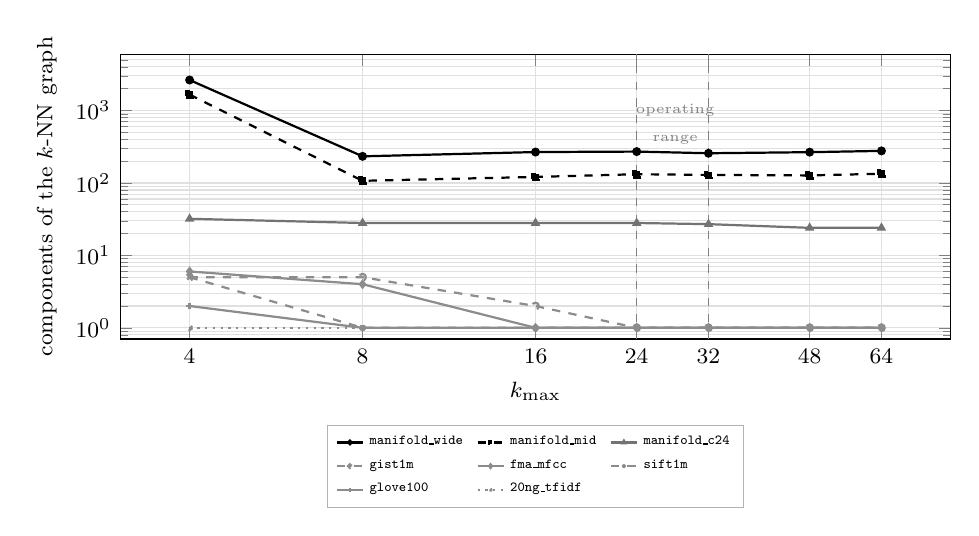
\begin{tikzpicture}
\begin{axis}[
  width=\columnwidth, height=5.2cm,
  xlabel={$\kmax$}, ylabel={components of the $k$-NN graph},
  ymode=log, log basis y=10,
  xmode=log, log basis x=2, xtick={4,8,16,24,32,48,64},
  xticklabels={4,8,16,24,32,48,64},
  ymin=0.7, ymax=6000,
  grid=both, grid style={black!12},
  legend style={font=\tiny, at={(0.5,-0.30)}, anchor=north,
                legend columns=3, draw=black!30, legend cell align=left,
                /tikz/every even column/.append style={column sep=1mm}},
  legend image post style={scale=0.55},
  label style={font=\footnotesize}, tick label style={font=\footnotesize},
  every axis plot/.append style={thick, mark size=1.2pt}
]
\addplot[mark=*, black] coordinates {(4,2636)(8,233)(16,267)(24,271)(32,257)(48,266)(64,277)};
\addlegendentry{\texttt{manifold\_wide}}
\addplot[mark=square*, black, dashed] coordinates {(4,1658)(8,107)(16,121)(24,132)(32,129)(48,127)(64,134)};
\addlegendentry{\texttt{manifold\_mid}}
\addplot[mark=triangle*, black!55] coordinates {(4,32)(8,28)(16,28)(24,28)(32,27)(48,24)(64,24)};
\addlegendentry{\texttt{manifold\_c24}}
\addplot[mark=o, black!45, dashed] coordinates {(4,5)(8,5)(16,2)(24,1)(32,1)(48,1)(64,1)};
\addlegendentry{\texttt{gist1m}}
\addplot[mark=diamond*, black!45] coordinates {(4,6)(8,4)(16,1)(24,1)(32,1)(48,1)(64,1)};
\addlegendentry{\texttt{fma\_mfcc}}
\addplot[mark=x, black!45, dashed] coordinates {(4,5)(8,1)(16,1)(24,1)(32,1)(48,1)(64,1)};
\addlegendentry{\texttt{sift1m}}
\addplot[mark=+, black!45] coordinates {(4,2)(8,1)(16,1)(24,1)(32,1)(48,1)(64,1)};
\addlegendentry{\texttt{glove100}}
\addplot[mark=asterisk, black!45, dotted] coordinates {(4,1)(8,1)(16,1)(24,1)(32,1)(48,1)(64,1)};
\addlegendentry{\texttt{20ng\_tfidf}}
\draw[gray, dashed] (axis cs:24,0.7) -- (axis cs:24,6000);
\draw[gray, dashed] (axis cs:32,0.7) -- (axis cs:32,6000);
\node[font=\tiny, gray, anchor=south] at (axis cs:28,620) {operating};
\node[font=\tiny, gray, anchor=north] at (axis cs:28,620) {range};
\end{axis}
\end{tikzpicture}
\caption{Components of the $k$-NN graph alone, full $n$, mean of 3 seeds. Every
real data set reaches a single component at $\kmax \le 24$; the synthetic
manifold sets never do. Ambient dimensionality does not explain the threshold:
\texttt{20ng\_tfidf} ($d=1000$) connects at $\kmax = 4$ while \texttt{gist1m}
($d=960$) requires $\kmax = 24$.}
\label{fig:components}
\end{figure}

Three observations follow.

\textbf{The MST acts as a guard against fragmentation rather than as essential
structure.} If the $k$-NN graph is already connected, the spanning tree in
\eqref{eq:coresg} adds no edges that the neighbourhoods have not already
supplied, so the union in \eqref{eq:coresg} equals its first term and the second
term can be omitted without changing any extracted clustering. This also
explains why an approximation as coarse as ours suffices on such data. Deriving
the component labelling costs 0.08 to 3.5\,ms across our data sets against 5.3
to 222\,ms of hubness and bridge work, a factor of 48 to 136, so testing
connectivity first and skipping the bridge computation when it holds costs
little.

\textbf{Ambient dimensionality does not predict the threshold.}
\texttt{20ng\_tfidf} at $d=1000$ connects at $\kmax=4$; \texttt{gist1m} at
$d=960$ requires $\kmax=24$. What distinguishes them is whether the data
contains genuinely density-separated components each holding many points, a
property our synthetic family has by construction, and real data, at these
scales, largely lacks.

The connectivity observed is not a residual error of NN-Descent in the form of
long cross-component edges that connect a graph an exact $k$-NN would leave in
pieces. At the operating $\kmax$: on \texttt{manifold\_c24} the exact graph
yields 24 components and the approximate graph 24 to 28, since a missed
neighbour removes an edge while a substituted one stays local. The effect does
reverse once $\kmax$ approaches the component size (\texttt{manifold\_c32} at
$\kmax=64$: 30 approximate against 32 exact), so we state the claim narrowly.

\subsection{Incremental Construction Beats a Compute-Matched Rebuild}
\label{sec:incremental}

Building on half the data and inserting the rest in eight batches, the
incremental graph has higher $k$-NN recall than a rebuild on the same final data
for all eight data sets tested. The incremental path revisits sampled base
points once per batch, so after eight batches the base has been refined eight
times, whereas a full rebuild performs a single construction from scratch.

Fig.~\ref{fig:frontier} therefore sweeps the effort given to that rebuild and
places the incremental result against the resulting frontier. \emph{Tuning} here
means raising two NN-Descent parameters of the rebuild: the number of descent
rounds, and the width of the candidate list examined per round. Each open marker
is one \textbf{alternative} rebuild configuration, an independent run of its
own; the markers are not cumulative and are not summed.

\begin{figure}[!t]
\centering
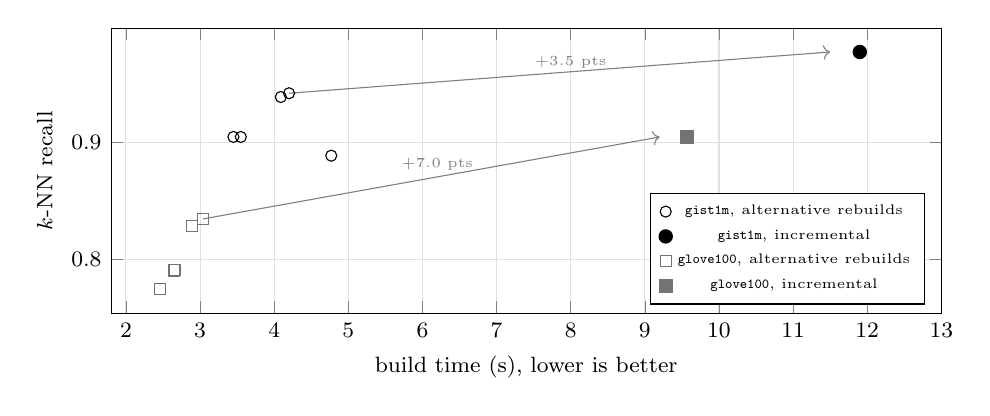
\begin{tikzpicture}
\begin{axis}[
  width=\columnwidth, height=5.2cm,
  xlabel={build time (s), lower is better},
  ylabel={$k$-NN recall},
  grid=both, grid style={black!12},
  legend style={font=\tiny, at={(0.98,0.03)}, anchor=south east},
  label style={font=\footnotesize}, tick label style={font=\footnotesize},
  xmin=1.8, xmax=13
]
\addplot[only marks, mark=o, black] coordinates {(4.77,0.88852)(3.55,0.90452)(3.45,0.90457)(4.09,0.93871)(4.20,0.94190)};
\addlegendentry{\texttt{gist1m}, alternative rebuilds}
\addplot[only marks, mark=*, black, mark size=2.4pt] coordinates {(11.90,0.97723)};
\addlegendentry{\texttt{gist1m}, incremental}
\addplot[only marks, mark=square, black!55] coordinates {(2.46,0.77413)(2.66,0.79043)(2.65,0.79032)(2.89,0.82866)(3.04,0.83441)};
\addlegendentry{\texttt{glove100}, alternative rebuilds}
\addplot[only marks, mark=square*, black!55, mark size=2.4pt] coordinates {(9.57,0.90451)};
\addlegendentry{\texttt{glove100}, incremental}
\draw[->, gray, thin] (axis cs:4.20,0.94190) -- (axis cs:11.5,0.97723);
\draw[->, gray, thin] (axis cs:3.04,0.83441) -- (axis cs:9.2,0.90451);
\node[font=\tiny, gray, anchor=south] at (axis cs:8.0,0.955) {$+3.5$ pts};
\node[font=\tiny, gray, anchor=south] at (axis cs:6.2,0.868) {$+7.0$ pts};
\end{axis}
\end{tikzpicture}
\caption{Quality against cost. Each open marker is one \emph{alternative}
rebuild configuration, run independently; they are not cumulative. Filled
markers are the incremental result. A single rebuild is cheaper in wall clock
than the incremental path, and remains lower in recall than it even when tuned:
margins of 3.5 and 7.0 percentage points survive against the best rebuild found.
Single RTX 4070 Ti SUPER; recall is hardware-independent.}
\label{fig:frontier}
\end{figure}

We conclude that:

\emph{Extra descent rounds do not substitute for a wider candidate list.} On
\texttt{gist1m}, doubling and then quadrupling the number of rounds \emph{of the
rebuild} returns bit-identical distance-evaluation counts, 222.5\,M in both
cases, because the early-stopping criterion fires at the same round either way.
A rebuild has reached a fixed point of the local join, so it is not short of
time and cannot be improved by being given more of it. Widening the candidate
list does help, raising recall from 0.88852 to 0.93871, since it changes which
pairs are compared. This matters for the comparison because it establishes that
the rebuild baseline was not simply under-resourced: it was given both kinds of
extra effort, and the better of the two was used.

\emph{A margin survives that tuning.} The best rebuild we found reaches 0.94190
on \texttt{gist1m} and 0.83441 on \texttt{glove100}, against 0.97723 and 0.90451
for the incremental graph, margins of 3.5 and 7.0 percentage points of $k$-NN
recall. Thus, incremental construction produces a better graph than a
compute-matched rebuild on data where a single construction pass struggles, and
the margin grows with the difficulty of the $k$-NN problem: $+0.09$ points on
\texttt{manifold\_mid}, $+3.5$ on \texttt{gist1m}, $+7.0$ on \texttt{glove100}.

These two observations together say that the advantage is real but is a quality
advantage, not a wall-clock one: a single rebuild is cheaper than the
incremental path in isolation. Cost-competitiveness comes from two other
directions, namely realistic batch sizes (Section~\ref{sec:batchsize}) and
multi-device execution (Section~\ref{sec:scaling}).

\subsection{Amortisation and Batch Size}
\label{sec:batchsize}

Fig.~\ref{fig:batch} sweeps the batch size, expressed as a fraction of the final
data set size $n$, against the cost of inserting one point.

\begin{figure}[!t]
\centering
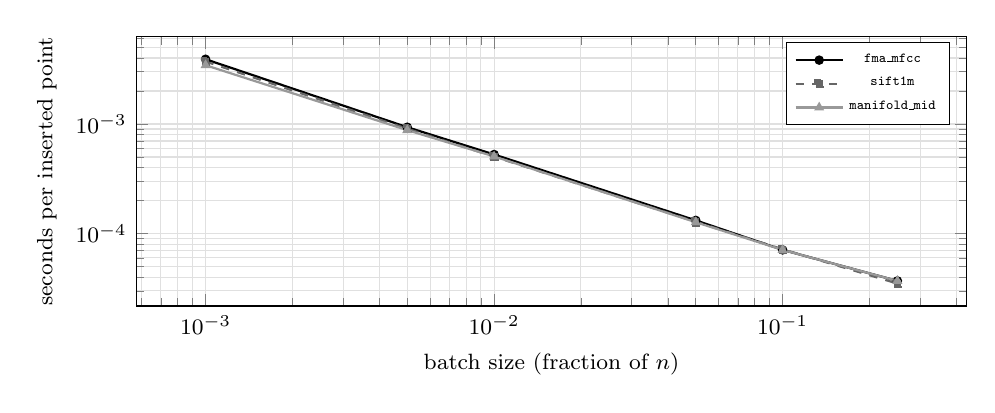
\begin{tikzpicture}
\begin{axis}[
  width=\columnwidth, height=5.0cm,
  xlabel={batch size (fraction of $n$)}, ylabel={seconds per inserted point},
  xmode=log, ymode=log,
  grid=both, grid style={black!12},
  legend style={font=\tiny, at={(0.98,0.98)}, anchor=north east},
  label style={font=\footnotesize}, tick label style={font=\footnotesize},
  every axis plot/.append style={thick, mark size=1.3pt}
]
\addplot[mark=*, black] coordinates {(0.001,0.003900)(0.005,0.000935)(0.010,0.000527)(0.050,0.000132)(0.100,0.000071)(0.250,0.000037)};
\addlegendentry{\texttt{fma\_mfcc}}
\addplot[mark=square*, black!60, dashed] coordinates {(0.001,0.003719)(0.005,0.000905)(0.010,0.000504)(0.050,0.000128)(0.100,0.000072)(0.250,0.000035)};
\addlegendentry{\texttt{sift1m}}
\addplot[mark=triangle*, black!40] coordinates {(0.001,0.003441)(0.005,0.000879)(0.010,0.000506)(0.050,0.000127)(0.100,0.000071)(0.250,0.000037)};
\addlegendentry{\texttt{manifold\_mid}}
\end{axis}
\end{tikzpicture}
\caption{Per-point update cost against batch size, $n = 50{,}000$, 3 seeds,
cluster hardware. For the three sets plotted, the fixed per-update phases,
namely the hubness refresh, bridge spanning tree and connectivity pass, rise
from 8.6 to 8.9\% of update time at a 25\% batch to 24.6 to 26.2\% at a 0.1\%
batch.}
\label{fig:batch}
\end{figure}

A batch of 0.1\% is one containing $0.001n$ points, so smaller batches mean more
frequent, smaller updates. \textbf{At a 25\% batch an incremental update costs
0.97 to 1.24 times a full rebuild and produces a better graph on all four data
sets tested}, by 0.4 to 5.9 percentage points of recall. At that batch size the
method is therefore free relative to the rebuild it replaces.

Smaller batches cost more per point: inserting at 0.1\% costs roughly 100 times
more per point than at 25\%, because the fixed phases of an update run once per
insertion regardless of how many points arrived. The recall gained in return is
at most 0.25 percentage points. The practical reading is that batches should be
as large as the application's latency budget allows, and that at 10 to 25\% of
the graph an update is effectively free.

\subsection{Multi-GPU Scaling}
\label{sec:scaling}

This is where the method's throughput advantage lies. Table~\ref{tab:scaling}
reports strong scaling with the instance count held fixed across device counts.

\begin{table}[!t]
\caption{Strong scaling with the instance count fixed at 16. $f$ is the
\emph{parallel fraction}, the share of update time spent in the instance phase,
which is the only phase distributed across devices; it is measured on the
single-device run. ``@4'' denotes four GPUs. The Amdahl ceiling is the maximum
speed-up attainable at four devices given $f$.}
\label{tab:scaling}
\centering
\footnotesize
\begin{tabular}{@{}lrrrrr@{}}
\toprule
data set & $n$ & $f$ & ceiling @4 & measured @4 & efficiency \\
\midrule
\texttt{capacity10m}  & 10\,M   & 0.941 & 3.40$\times$ & \textbf{3.23}$\times$ & 0.81 \\
\texttt{gist1m}       & 100\,k  & 0.921 & 3.23$\times$ & \textbf{2.68}$\times$ & 0.67 \\
\texttt{sift1m}       & 200\,k  & 0.869 & 2.87$\times$ & \textbf{2.53}$\times$ & 0.63 \\
\texttt{manifold\_mid}& 100\,k  & 0.840 & 2.70$\times$ & \textbf{2.50}$\times$ & 0.63 \\
\bottomrule
\end{tabular}
\end{table}

Every measurement sits below its Amdahl ceiling \cite{amdahl}, and
\textbf{efficiency rises with problem size}, from 0.63 at $n = 10^5$ to 0.81 at
$n = 10^7$, because larger instances amortise the fixed per-job transfer. The
largest configuration reaches \textbf{3.23 times} the single-device throughput
on four GPUs. This trend is the strongest form of the scalability argument: the
method does not merely tolerate more devices, it uses them better as the problem
grows, which is the regime the design targets.

Note that $f$ is measured on the single-device run, and falls as devices are
added, from 0.941 to 0.798 between one and four GPUs on \texttt{capacity10m},
because the instance phase is exactly the part being parallelised and therefore
shrinks. Taking $f$ from a parallel run would understate the ceiling and make
every measurement appear to exceed it.

Two further results characterise the design. \textbf{Parallelism is bounded by
the decomposition}: with a single instance, four GPUs deliver 0.99$\times$, while
with two the speed-up appears at two devices and plateaus where the instances run
out. \textbf{Per-device memory is exactly invariant with device count} and
controlled entirely by the instance count (Fig.~\ref{fig:memory}). The response
to a data set that does not fit is therefore to re-partition on the same
hardware rather than to add devices or memory; a design that replicated data
across devices, or whose per-device state grew with the device count, would not
have this property. At $\kmax=128$ one instance over $10^7$ points requires
8.29\,GiB and an 8\,GB device refuses it, matching our sizing model's
prediction.

\begin{figure}[!t]
\centering
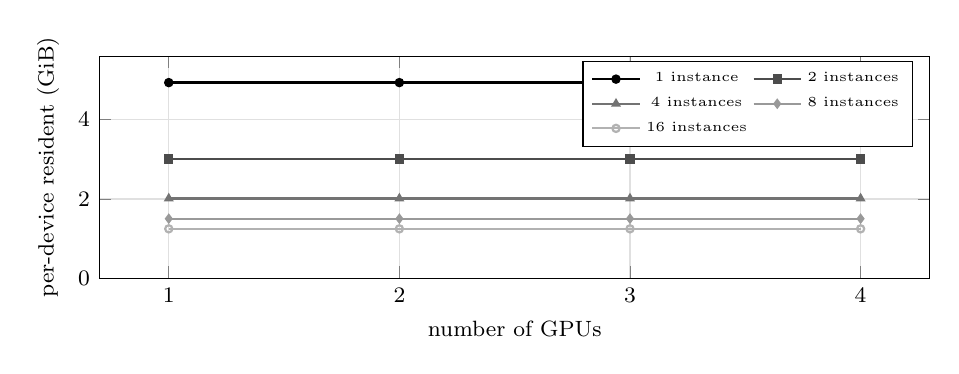
\begin{tikzpicture}
\begin{axis}[
  width=\columnwidth, height=4.4cm,
  xlabel={number of GPUs}, ylabel={per-device resident (GiB)},
  xtick={1,2,3,4}, ymin=0, ymax=5.6,
  grid=both, grid style={black!12},
  legend style={font=\tiny, at={(0.98,0.98)}, anchor=north east, legend columns=2},
  label style={font=\footnotesize}, tick label style={font=\footnotesize},
  every axis plot/.append style={thick, mark size=1.3pt}
]
\addplot[mark=*, black] coordinates {(1,4.936)(2,4.936)(3,4.936)(4,4.936)};
\addlegendentry{1 instance}
\addplot[mark=square*, black!70] coordinates {(1,3.010)(2,3.010)(3,3.010)(4,3.010)};
\addlegendentry{2 instances}
\addplot[mark=triangle*, black!55] coordinates {(1,2.011)(2,2.011)(3,2.011)(4,2.011)};
\addlegendentry{4 instances}
\addplot[mark=diamond*, black!40] coordinates {(1,1.502)(2,1.502)(3,1.502)(4,1.502)};
\addlegendentry{8 instances}
\addplot[mark=o, black!30] coordinates {(1,1.246)(2,1.246)(3,1.246)(4,1.246)};
\addlegendentry{16 instances}
\end{axis}
\end{tikzpicture}
\caption{Per-device memory on \texttt{capacity10m} ($10^7$ points), flat across
device count and set entirely by the instance count.}
\label{fig:memory}
\end{figure}

Two further time savings are worth recording alongside the scaling result.
Bridge construction is 10.5 to 36 times faster than the exact spanning tree it
replaces (Table~\ref{tab:bridges}). And extracting all 32 spanning trees for
$\mpts \in [1,\kmax]$ from one CORE-SG costs 71 to 303 times less than computing
each from the complete graph, a payoff that is preserved after incremental
construction.

\subsection{Comparison with FISHDBC}
\label{sec:fishdbc}

We drive both methods over one arrival order, export our spanning tree per
batch, and convert it to HDBSCAN* labels using the same condensed-tree
extraction FISHDBC itself calls, scoring both against one reference: exact
HDBSCAN* recomputed on the points present at that batch. The only quantity that
differs between the two rows is the spanning tree each method produced.

\begin{table}[!t]
\caption{ARI against exact HDBSCAN* on the points present at each batch.
20{,}000 points, 8 batches, $\mpts=10$, 2 seeds.}
\label{tab:fishdbc}
\centering
\footnotesize
\begin{tabular}{@{}lccc@{}}
\toprule
data set & this work & FISHDBC & margin \\
\midrule
\texttt{manifold\_mid} & \textbf{1.0000} (all 8) & 0.9925--0.9962 & $+0.004$--$0.008$ \\
\texttt{sift1m}        & 0.9920--0.9980 & 0.9745--0.9855 & $+0.009$--$0.022$ \\
\bottomrule
\end{tabular}
\end{table}

Our method is ahead on every batch of each data set (Table~\ref{tab:fishdbc})
and recovers the reference clustering exactly at every point of the
\texttt{manifold\_mid} stream. We exclude \texttt{fma\_mfcc}: its reference
finds only two clusters until batch five and both methods' ARI collapses to
approximately 0.09 as it destabilises, so the data set cannot support a quality
claim in either direction, though the two methods agree with each other to
within 0.014 throughout. And we do not compare wall-clock: FISHDBC is
single-threaded Python against our C++/CUDA, so only the cost \emph{slope} is
meaningful. As the graph doubled, per-batch cost grew 1.10 to 1.27 times for our
method against 0.93 to 1.17 for FISHDBC, comparable, with a slight structural
edge to FISHDBC, whose index insertion is $O(\log n)$ per point.

Only one external method is compared because only one satisfies the two criteria
in Section~\ref{sec:setup}: maintenance under insertion, at the granularity of
individual points. The alternatives either operate over summaries or have no
update path at all.

The two methods also differ in scope. FISHDBC serves a single $\mpts$, whereas
the CORE-SG serves the whole range from one graph.

\subsection{Parameter Sensitivity}
\label{sec:sensitivity}

Anti-hub coverage parameters produce no signal on data whose $k$-NN graph is
connected, which, per Section~\ref{sec:connectivity}, is every real data set.
Re-run on fragmenting data the result is positive. The \emph{per-component
quota} is the minimum number of anti-hubs each $k$-NN component contributes
regardless of the global selection, introduced in Section~\ref{sec:bridges} to
stop small components being passed over. On \texttt{manifold\_wide}, 300
components are reduced to one even when the anti-hub count is halved and the
quota is switched off entirely.

The anti-hub count's dimensionality term matters more. The \emph{ambient
dimensionality} $d$ is the number of coordinates each point carries, as opposed
to the intrinsic dimensionality of the manifold the data occupies. In our
experiments, using ambient $d$ in $\lceil d \ln|E| \rceil$ selected 100\% of the
points on the two data sets with $d \ge 500$, so the estimate degenerated into
the exact MST, and 18 to 40\% on the remaining data sets, which is not sublinear
in any useful sense. Substituting it with an intrinsic dimensionality estimated
free from the stored $k$-NN radii \cite{levina_bickel}, pooled with the harmonic
mean \cite{mackay_ghahramani}, uses 1.4 to 11.8\% and runs 3.2 to 35.9 times
faster, at a cost of at most 0.5\% in spanning-tree weight where bridges are
load-bearing.

The \emph{refinement cap} bounds how many nodes may participate in the
restricted descent that follows a batch (Section~\ref{sec:knn}); a larger cap
lets more existing points revise their neighbour lists after new data arrives.
Quality is monotone in that cap, and how much it matters is a property of the
data: 0.007 percentage points of recall on \texttt{fma\_mfcc} against 0.72 on
\texttt{manifold\_wide}, for 0.6\% more time. The cap is expressed as a fraction
of $n$, which makes the cost of an update linear in $n$ against the quadratic
cost of the rebuild it replaces. Expressing it instead as an absolute ceiling
would tie the refinement set to the batch size alone, and whether that retains
quality as $n$ grows is a question left open. All reported results use the same
shipped value.

% ===========================================================================
\section{Conclusion and Future Work}
% ===========================================================================

We have made the CORE-SG incremental and multi-GPU by attacking its two
constituent graphs separately: sampled-instance dynamic NN-Descent for the
neighbourhood graph, and an anti-hub bridge estimate for the spanning tree whose
selected set is sized independently of $n$ and therefore requires no incremental
maintenance.

The estimate produces spanning trees at most 0.024\% heavier than exact at ARI
exactly 1.0000, while building 10.5 to 36 times faster than the exact spanning
tree it replaces. Incremental construction produces a better graph than a
compute-matched rebuild, by up to 7.0 percentage points of recall, and at a 25\%
batch it costs 0.97 to 1.24 times a single rebuild while remaining more
accurate. On the time axis the strongest result is distribution: four GPUs
deliver 3.23 times the single-device throughput at $10^7$ points, with
efficiency \emph{rising} with problem size and per-device memory exactly
invariant with device count, so larger problems are served better by more
devices rather than worse. Extracting the whole $\mpts$ range from one graph
remains 71 to 303 times cheaper than recomputing each, and that payoff survives
incremental construction. Against the closest published incremental method the
approach is ahead on every batch tested, while additionally serving a range of
$\mpts$ for which that method has no equivalent.

Several directions follow.

\textbf{Is the spanning tree needed on real data at all?} Real $k$-NN graphs are
already connected at the operating $\kmax$, which suggests that for a large
class of real data the single-linkage structure is recoverable from the
neighbourhood graph alone, with the spanning tree required only as a guard.
Characterising which data requires it, and detecting that cheaply as our
connectivity check does, would simplify density-based clustering pipelines
beyond this system.

\textbf{Sampled-instance descent as a construction method.}
Section~\ref{sec:incremental} shows overlapping sampled instances beating a
single construction pass at matched compute. Studied on its own, varying the
instance count, the overlap fraction and the number of passes, this may be a
better way to build large $k$-NN graphs, independent of incrementality.

\textbf{Intrinsic dimensionality as a general parameter scale.} The anti-hub
count was one instance of a broader pattern: any parameter in a density-based
method that scales with ambient $d$ deserves the same scrutiny.

\textbf{The form of the refinement cap}, discussed in
Section~\ref{sec:sensitivity}.

\textbf{Multi-node execution and deletion.} The instance abstraction is already
the right unit to ship to another machine, and top-$k$ merging is a commutative,
associative reduction, so it distributes without synchronisation; because the
anti-hub set is sized independently of $n$, the bridge spanning tree can be
gathered onto one machine at any scale. Deletion is untouched and is the harder
direction.

\section*{Acknowledgment}
TODO.

\bibliographystyle{IEEEtran}
\bibliography{references}

\EOD

\end{document}
